\section{Model Checking the CCUCprotocol}
This section will utilise UPPAAL to see what happens with the model when unreliability is introduced to the model.

The changes to the model are that whenever something is received, it will have a chance to miss the transmission, and therefore not fire the edge which receives the transmission.
This can be modelled in UPPAAL using the branch points as seen on \myref{fig:missTransmission}.

\begin{wrapfigure}{R}{0.3\textwidth}
\centering
  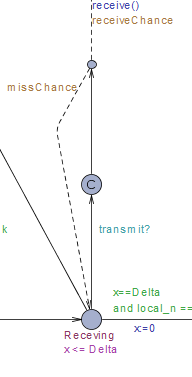
\includegraphics[width=0.3\textwidth]{Figures/Model/MissChance.png} 
\caption{Graph showing the split node after receiving, where there is a chance for the device to miss the transmission and go back to the same location.}
\label{fig:missTransmission}
\end{wrapfigure}

The chances \texttt{missChance} and \texttt{receiveChance} are simply created so the sum of them is 100 and this is shown in 

\begin{lstlisting}[style=UPPAAL, title={The creation of }]
4. Pr[<=300000] Pr[<=300000] ( <>  forall(i : id_t) (time >3000) 
    and Device(i).local_n == N + 1)
\end{lstlisting}
